% Created by tikzDevice version 0.6.4 on 2013-12-01 11:37:16
% !TEX encoding = UTF-8 Unicode
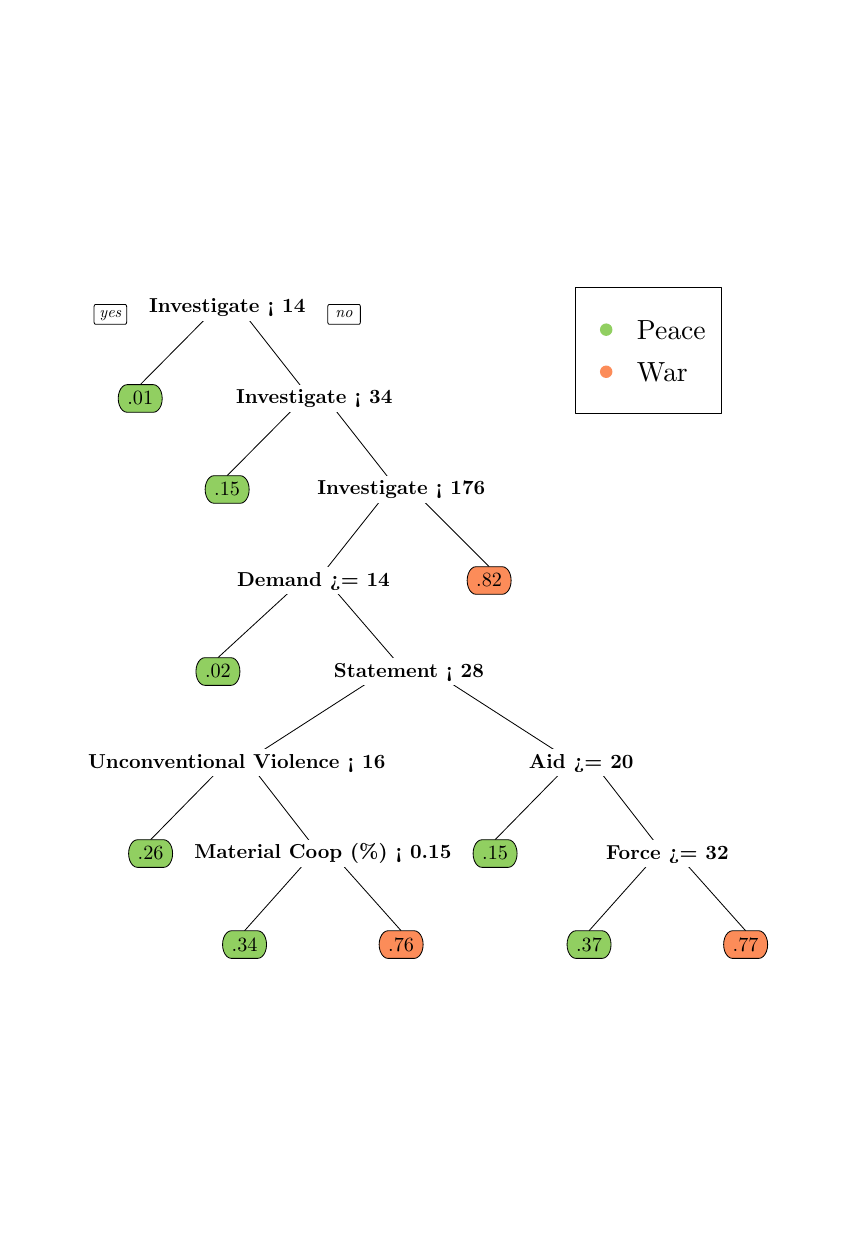
\begin{tikzpicture}[x=1pt,y=1pt]
\definecolor[named]{fillColor}{rgb}{1.00,1.00,1.00}
\path[use as bounding box,fill=fillColor,fill opacity=0.00] (0,0) rectangle (289.08,433.62);
\begin{scope}
\path[clip] (  0.00,  0.00) rectangle (289.08,433.62);
\definecolor[named]{drawColor}{rgb}{0.00,0.00,0.00}

\path[draw=drawColor,line width= 0.3pt,line join=round] ( 40.67,304.62) --
	( 65.82,330.02) --
	( 72.11,330.02);

\path[draw=drawColor,line width= 0.3pt,line join=round] (103.54,297.96) --
	( 78.39,330.02) --
	( 72.11,330.02);

\path[draw=drawColor,line width= 0.3pt,line join=round] ( 72.08,271.73) --
	( 97.25,297.13) --
	(103.54,297.13);

\path[draw=drawColor,line width= 0.3pt,line join=round] (135.01,265.07) --
	(109.84,297.13) --
	(103.54,297.13);

\path[draw=drawColor,line width= 0.3pt,line join=round] (103.27,232.19) --
	(128.66,264.24) --
	(135.01,264.24);

\path[draw=drawColor,line width= 0.3pt,line join=round] ( 68.75,205.96) --
	( 96.36,231.35) --
	(103.27,231.35);

\path[draw=drawColor,line width= 0.3pt,line join=round] (137.78,199.30) --
	(110.17,231.35) --
	(103.27,231.35);

\path[draw=drawColor,line width= 0.3pt,line join=round] ( 75.54,166.41) --
	(125.33,198.47) --
	(137.78,198.47);

\path[draw=drawColor,line width= 0.3pt,line join=round] ( 44.42,140.18) --
	( 69.32,165.58) --
	( 75.54,165.58);

\path[draw=drawColor,line width= 0.3pt,line join=round] (106.66,133.52) --
	( 81.76,165.58) --
	( 75.54,165.58);

\path[draw=drawColor,line width= 0.3pt,line join=round] ( 78.37,107.29) --
	(101.00,132.69) --
	(106.66,132.69);

\path[draw=drawColor,line width= 0.3pt,line join=round] (134.95,107.29) --
	(112.32,132.69) --
	(106.66,132.69);

\path[draw=drawColor,line width= 0.3pt,line join=round] (200.02,166.41) --
	(150.23,198.47) --
	(137.78,198.47);

\path[draw=drawColor,line width= 0.3pt,line join=round] (168.90,140.18) --
	(193.80,165.58) --
	(200.02,165.58);

\path[draw=drawColor,line width= 0.3pt,line join=round] (231.14,133.52) --
	(206.25,165.58) --
	(200.02,165.58);

\path[draw=drawColor,line width= 0.3pt,line join=round] (202.85,107.29) --
	(225.48,132.69) --
	(231.14,132.69);

\path[draw=drawColor,line width= 0.3pt,line join=round] (259.43,107.29) --
	(236.80,132.69) --
	(231.14,132.69);

\path[draw=drawColor,line width= 0.3pt,line join=round] (166.75,238.84) --
	(141.36,264.24) --
	(135.01,264.24);
\definecolor[named]{fillColor}{rgb}{1.00,1.00,1.00}

\path[fill=fillColor] ( 38.12,327.52) --
	( 38.12,337.52) --
	(106.09,337.52) --
	(106.09,327.52) --
	( 38.12,327.52) --
	cycle;

\path[fill=fillColor] ( 69.56,294.63) --
	( 69.56,304.64) --
	(137.52,304.64) --
	(137.52,294.63) --
	( 69.56,294.63) --
	cycle;

\path[fill=fillColor] ( 98.94,261.74) --
	( 98.94,271.75) --
	(171.07,271.75) --
	(171.07,261.74) --
	( 98.94,261.74) --
	cycle;

\path[fill=fillColor] ( 70.64,228.85) --
	( 70.64,238.86) --
	(135.89,238.86) --
	(135.89,228.85) --
	( 70.64,228.85) --
	cycle;

\path[fill=fillColor] (104.94,195.96) --
	(104.94,205.97) --
	(170.62,205.97) --
	(170.62,195.96) --
	(104.94,195.96) --
	cycle;

\path[fill=fillColor] ( 16.26,163.08) --
	( 16.26,173.08) --
	(134.83,173.08) --
	(134.83,163.08) --
	( 16.26,163.08) --
	cycle;

\path[fill=fillColor] ( 54.60,130.19) --
	( 54.60,140.19) --
	(158.72,140.19) --
	(158.72,130.19) --
	( 54.60,130.19) --
	cycle;

\path[fill=fillColor] (176.01,163.08) --
	(176.01,173.08) --
	(224.03,173.08) --
	(224.03,163.08) --
	(176.01,163.08) --
	cycle;

\path[fill=fillColor] (203.92,130.19) --
	(203.92,140.19) --
	(258.37,140.19) --
	(258.37,130.19) --
	(203.92,130.19) --
	cycle;

\node[text=drawColor,anchor=base,inner sep=0pt, outer sep=0pt, scale=  0.73] at ( 72.11,330.72) {\bfseries Investigate < 14};

\node[text=drawColor,anchor=base,inner sep=0pt, outer sep=0pt, scale=  0.73] at (103.54,297.84) {\bfseries Investigate < 34};

\node[text=drawColor,anchor=base,inner sep=0pt, outer sep=0pt, scale=  0.73] at (135.01,264.95) {\bfseries Investigate < 176};

\node[text=drawColor,anchor=base,inner sep=0pt, outer sep=0pt, scale=  0.73] at (103.27,231.71) {\bfseries Demand >= 14};

\node[text=drawColor,anchor=base,inner sep=0pt, outer sep=0pt, scale=  0.73] at (137.78,198.82) {\bfseries Statement < 28};

\node[text=drawColor,anchor=base,inner sep=0pt, outer sep=0pt, scale=  0.73] at ( 75.54,165.93) {\bfseries Unconventional Violence < 16};

\node[text=drawColor,anchor=base,inner sep=0pt, outer sep=0pt, scale=  0.73] at (106.66,133.38) {\bfseries Material Coop (\%) < 0.15};

\node[text=drawColor,anchor=base,inner sep=0pt, outer sep=0pt, scale=  0.73] at (200.02,165.93) {\bfseries Aid >= 20};

\node[text=drawColor,anchor=base,inner sep=0pt, outer sep=0pt, scale=  0.73] at (231.14,133.04) {\bfseries Force >= 32};
\definecolor[named]{fillColor}{rgb}{0.57,0.81,0.38}

\path[draw=drawColor,line width= 0.3pt,line join=round,line cap=round,fill=fillColor] ( 32.71,299.63) --
	( 32.82,300.92) --
	( 33.15,302.12) --
	( 33.66,303.16) --
	( 34.33,303.95) --
	( 35.11,304.45) --
	( 35.95,304.62) --
	( 45.39,304.62) --
	( 46.23,304.45) --
	( 47.00,303.95) --
	( 47.67,303.16) --
	( 48.19,302.12) --
	( 48.51,300.92) --
	( 48.62,299.63) --
	( 48.62,299.63) --
	( 48.51,298.34) --
	( 48.19,297.13) --
	( 47.67,296.10) --
	( 47.00,295.30) --
	( 46.23,294.80) --
	( 45.39,294.63) --
	( 35.95,294.63) --
	( 35.11,294.80) --
	( 34.33,295.30) --
	( 33.66,296.10) --
	( 33.15,297.13) --
	( 32.82,298.34) --
	( 32.71,299.63) --
	cycle;

\path[draw=drawColor,line width= 0.3pt,line join=round,line cap=round,fill=fillColor] ( 64.12,266.74) --
	( 64.23,268.03) --
	( 64.56,269.24) --
	( 65.07,270.27) --
	( 65.74,271.06) --
	( 66.52,271.56) --
	( 67.36,271.73) --
	( 76.80,271.73) --
	( 77.64,271.56) --
	( 78.41,271.06) --
	( 79.08,270.27) --
	( 79.60,269.24) --
	( 79.92,268.03) --
	( 80.03,266.74) --
	( 80.03,266.74) --
	( 79.92,265.45) --
	( 79.60,264.24) --
	( 79.08,263.21) --
	( 78.41,262.42) --
	( 77.64,261.92) --
	( 76.80,261.75) --
	( 67.36,261.75) --
	( 66.52,261.92) --
	( 65.74,262.42) --
	( 65.07,263.21) --
	( 64.56,264.24) --
	( 64.23,265.45) --
	( 64.12,266.74) --
	cycle;

\path[draw=drawColor,line width= 0.3pt,line join=round,line cap=round,fill=fillColor] ( 60.80,200.96) --
	( 60.91,202.26) --
	( 61.23,203.46) --
	( 61.74,204.49) --
	( 62.41,205.29) --
	( 63.19,205.79) --
	( 64.03,205.96) --
	( 73.47,205.96) --
	( 74.31,205.79) --
	( 75.09,205.29) --
	( 75.76,204.49) --
	( 76.27,203.46) --
	( 76.59,202.26) --
	( 76.70,200.96) --
	( 76.70,200.96) --
	( 76.59,199.67) --
	( 76.27,198.47) --
	( 75.76,197.43) --
	( 75.09,196.64) --
	( 74.31,196.14) --
	( 73.47,195.97) --
	( 64.03,195.97) --
	( 63.19,196.14) --
	( 62.41,196.64) --
	( 61.74,197.43) --
	( 61.23,198.47) --
	( 60.91,199.67) --
	( 60.80,200.96) --
	cycle;

\path[draw=drawColor,line width= 0.3pt,line join=round,line cap=round,fill=fillColor] ( 36.47,135.19) --
	( 36.58,136.48) --
	( 36.90,137.68) --
	( 37.41,138.72) --
	( 38.08,139.51) --
	( 38.86,140.01) --
	( 39.70,140.18) --
	( 49.14,140.18) --
	( 49.98,140.01) --
	( 50.76,139.51) --
	( 51.43,138.72) --
	( 51.94,137.68) --
	( 52.26,136.48) --
	( 52.37,135.19) --
	( 52.37,135.19) --
	( 52.26,133.89) --
	( 51.94,132.69) --
	( 51.43,131.66) --
	( 50.76,130.86) --
	( 49.98,130.36) --
	( 49.14,130.19) --
	( 39.70,130.19) --
	( 38.86,130.36) --
	( 38.08,130.86) --
	( 37.41,131.66) --
	( 36.90,132.69) --
	( 36.58,133.89) --
	( 36.47,135.19) --
	cycle;

\path[draw=drawColor,line width= 0.3pt,line join=round,line cap=round,fill=fillColor] ( 70.42,102.30) --
	( 70.53,103.59) --
	( 70.85,104.79) --
	( 71.36,105.83) --
	( 72.03,106.62) --
	( 72.81,107.12) --
	( 73.65,107.29) --
	( 83.09,107.29) --
	( 83.93,107.12) --
	( 84.71,106.62) --
	( 85.38,105.83) --
	( 85.89,104.79) --
	( 86.21,103.59) --
	( 86.32,102.30) --
	( 86.32,102.30) --
	( 86.21,101.01) --
	( 85.89, 99.80) --
	( 85.38, 98.77) --
	( 84.71, 97.97) --
	( 83.93, 97.47) --
	( 83.09, 97.30) --
	( 73.65, 97.30) --
	( 72.81, 97.47) --
	( 72.03, 97.97) --
	( 71.36, 98.77) --
	( 70.85, 99.80) --
	( 70.53,101.01) --
	( 70.42,102.30) --
	cycle;
\definecolor[named]{fillColor}{rgb}{0.99,0.55,0.35}

\path[draw=drawColor,line width= 0.3pt,line join=round,line cap=round,fill=fillColor] (127.00,102.30) --
	(127.11,103.59) --
	(127.43,104.79) --
	(127.95,105.83) --
	(128.61,106.62) --
	(129.39,107.12) --
	(130.23,107.29) --
	(139.67,107.29) --
	(140.51,107.12) --
	(141.29,106.62) --
	(141.96,105.83) --
	(142.47,104.79) --
	(142.79,103.59) --
	(142.90,102.30) --
	(142.90,102.30) --
	(142.79,101.01) --
	(142.47, 99.80) --
	(141.96, 98.77) --
	(141.29, 97.97) --
	(140.51, 97.47) --
	(139.67, 97.30) --
	(130.23, 97.30) --
	(129.39, 97.47) --
	(128.61, 97.97) --
	(127.95, 98.77) --
	(127.43, 99.80) --
	(127.11,101.01) --
	(127.00,102.30) --
	cycle;
\definecolor[named]{fillColor}{rgb}{0.57,0.81,0.38}

\path[draw=drawColor,line width= 0.3pt,line join=round,line cap=round,fill=fillColor] (160.95,135.19) --
	(161.06,136.48) --
	(161.38,137.68) --
	(161.89,138.72) --
	(162.56,139.51) --
	(163.34,140.01) --
	(164.18,140.18) --
	(173.62,140.18) --
	(174.46,140.01) --
	(175.24,139.51) --
	(175.91,138.72) --
	(176.42,137.68) --
	(176.74,136.48) --
	(176.85,135.19) --
	(176.85,135.19) --
	(176.74,133.89) --
	(176.42,132.69) --
	(175.91,131.66) --
	(175.24,130.86) --
	(174.46,130.36) --
	(173.62,130.19) --
	(164.18,130.19) --
	(163.34,130.36) --
	(162.56,130.86) --
	(161.89,131.66) --
	(161.38,132.69) --
	(161.06,133.89) --
	(160.95,135.19) --
	cycle;

\path[draw=drawColor,line width= 0.3pt,line join=round,line cap=round,fill=fillColor] (194.90,102.30) --
	(195.01,103.59) --
	(195.33,104.79) --
	(195.84,105.83) --
	(196.51,106.62) --
	(197.29,107.12) --
	(198.13,107.29) --
	(207.57,107.29) --
	(208.41,107.12) --
	(209.19,106.62) --
	(209.86,105.83) --
	(210.37,104.79) --
	(210.69,103.59) --
	(210.80,102.30) --
	(210.80,102.30) --
	(210.69,101.01) --
	(210.37, 99.80) --
	(209.86, 98.77) --
	(209.19, 97.97) --
	(208.41, 97.47) --
	(207.57, 97.30) --
	(198.13, 97.30) --
	(197.29, 97.47) --
	(196.51, 97.97) --
	(195.84, 98.77) --
	(195.33, 99.80) --
	(195.01,101.01) --
	(194.90,102.30) --
	cycle;
\definecolor[named]{fillColor}{rgb}{0.99,0.55,0.35}

\path[draw=drawColor,line width= 0.3pt,line join=round,line cap=round,fill=fillColor] (251.48,102.30) --
	(251.59,103.59) --
	(251.91,104.79) --
	(252.43,105.83) --
	(253.10,106.62) --
	(253.88,107.12) --
	(254.71,107.29) --
	(264.16,107.29) --
	(264.99,107.12) --
	(265.77,106.62) --
	(266.44,105.83) --
	(266.95,104.79) --
	(267.28,103.59) --
	(267.39,102.30) --
	(267.39,102.30) --
	(267.28,101.01) --
	(266.95, 99.80) --
	(266.44, 98.77) --
	(265.77, 97.97) --
	(264.99, 97.47) --
	(264.16, 97.30) --
	(254.71, 97.30) --
	(253.88, 97.47) --
	(253.10, 97.97) --
	(252.43, 98.77) --
	(251.91, 99.80) --
	(251.59,101.01) --
	(251.48,102.30) --
	cycle;

\path[draw=drawColor,line width= 0.3pt,line join=round,line cap=round,fill=fillColor] (158.80,233.85) --
	(158.91,235.14) --
	(159.23,236.35) --
	(159.74,237.38) --
	(160.41,238.18) --
	(161.19,238.67) --
	(162.03,238.84) --
	(171.47,238.84) --
	(172.31,238.67) --
	(173.09,238.18) --
	(173.76,237.38) --
	(174.27,236.35) --
	(174.59,235.14) --
	(174.70,233.85) --
	(174.70,233.85) --
	(174.59,232.56) --
	(174.27,231.35) --
	(173.76,230.32) --
	(173.09,229.53) --
	(172.31,229.03) --
	(171.47,228.86) --
	(162.03,228.86) --
	(161.19,229.03) --
	(160.41,229.53) --
	(159.74,230.32) --
	(159.23,231.35) --
	(158.91,232.56) --
	(158.80,233.85) --
	cycle;

\node[text=drawColor,anchor=base,inner sep=0pt, outer sep=0pt, scale=  0.73] at ( 40.67,297.30) {.01};

\node[text=drawColor,anchor=base,inner sep=0pt, outer sep=0pt, scale=  0.73] at ( 72.08,264.41) {.15};

\node[text=drawColor,anchor=base,inner sep=0pt, outer sep=0pt, scale=  0.73] at ( 68.75,198.64) {.02};

\node[text=drawColor,anchor=base,inner sep=0pt, outer sep=0pt, scale=  0.73] at ( 44.42,132.86) {.26};

\node[text=drawColor,anchor=base,inner sep=0pt, outer sep=0pt, scale=  0.73] at ( 78.37, 99.97) {.34};

\node[text=drawColor,anchor=base,inner sep=0pt, outer sep=0pt, scale=  0.73] at (134.95, 99.97) {.76};

\node[text=drawColor,anchor=base,inner sep=0pt, outer sep=0pt, scale=  0.73] at (168.90,132.86) {.15};

\node[text=drawColor,anchor=base,inner sep=0pt, outer sep=0pt, scale=  0.73] at (202.85, 99.97) {.37};

\node[text=drawColor,anchor=base,inner sep=0pt, outer sep=0pt, scale=  0.73] at (259.43, 99.97) {.77};

\node[text=drawColor,anchor=base,inner sep=0pt, outer sep=0pt, scale=  0.73] at (166.75,231.53) {.82};
\definecolor[named]{fillColor}{rgb}{1.00,1.00,1.00}

\path[draw=drawColor,line width= 0.3pt,line join=round,line cap=round,fill=fillColor] ( 23.99,332.72) --
	( 24.01,332.95) --
	( 24.06,333.17) --
	( 24.16,333.35) --
	( 24.28,333.49) --
	( 24.42,333.58) --
	( 24.57,333.61) --
	( 35.19,333.61) --
	( 35.34,333.58) --
	( 35.48,333.49) --
	( 35.60,333.35) --
	( 35.69,333.17) --
	( 35.75,332.95) --
	( 35.77,332.72) --
	( 35.77,327.32) --
	( 35.75,327.09) --
	( 35.69,326.87) --
	( 35.60,326.69) --
	( 35.48,326.54) --
	( 35.34,326.46) --
	( 35.19,326.42) --
	( 24.57,326.42) --
	( 24.42,326.46) --
	( 24.28,326.54) --
	( 24.16,326.69) --
	( 24.06,326.87) --
	( 24.01,327.09) --
	( 23.99,327.32) --
	cycle;

\path[draw=drawColor,line width= 0.3pt,line join=round,line cap=round,fill=fillColor] (108.44,332.72) --
	(108.46,332.95) --
	(108.52,333.17) --
	(108.61,333.35) --
	(108.73,333.49) --
	(108.87,333.58) --
	(109.02,333.61) --
	(119.64,333.61) --
	(119.79,333.58) --
	(119.93,333.49) --
	(120.05,333.35) --
	(120.15,333.17) --
	(120.20,332.95) --
	(120.22,332.72) --
	(120.22,327.32) --
	(120.20,327.09) --
	(120.15,326.87) --
	(120.05,326.69) --
	(119.93,326.54) --
	(119.79,326.46) --
	(119.64,326.42) --
	(109.02,326.42) --
	(108.87,326.46) --
	(108.73,326.54) --
	(108.61,326.69) --
	(108.52,326.87) --
	(108.46,327.09) --
	(108.44,327.32) --
	cycle;

\node[text=drawColor,anchor=base,inner sep=0pt, outer sep=0pt, scale=  0.58] at ( 29.88,328.74) {\itshape yes};

\node[text=drawColor,anchor=base,inner sep=0pt, outer sep=0pt, scale=  0.58] at (114.33,328.77) {\itshape no};
\end{scope}
\begin{scope}
\path[clip] ( 49.20, 61.20) rectangle (263.88,384.42);
\definecolor[named]{drawColor}{rgb}{0.00,0.00,0.00}

\path[draw=drawColor,line width= 0.4pt,line join=round,line cap=round] (197.93,339.70) rectangle (250.57,294.07);
\definecolor[named]{fillColor}{rgb}{0.57,0.81,0.38}

\path[fill=fillColor] (209.05,324.49) circle (  2.25);
\definecolor[named]{fillColor}{rgb}{0.99,0.55,0.35}

\path[fill=fillColor] (209.05,309.28) circle (  2.25);

\node[text=drawColor,anchor=base west,inner sep=0pt, outer sep=0pt, scale=  1.00] at (220.16,321.04) {Peace};

\node[text=drawColor,anchor=base west,inner sep=0pt, outer sep=0pt, scale=  1.00] at (220.16,305.84) {War};
\end{scope}
\end{tikzpicture}
